\documentclass[11pt]{standalone}
\usepackage{amssymb}
\usepackage{amsmath}
\usepackage[no-math]{fontspec}
\usepackage{unicode-math}
\setmainfont{Libertinus Sans}
\setsansfont{Libertinus Sans}
\setmathfont{Libertinus Math}
\usepackage{pgf,xcolor}
\usepackage{tikz}
\usetikzlibrary{arrows.meta, backgrounds, calc}
\usepackage{pgfplots}
\pgfplotsset{compat=newest}
\usepackage{pifont}

\definecolor{my_darkgray}{HTML}{484949}
\definecolor{my_lightgray}{HTML}{F3F4F4}
\definecolor{my_darkblue}{HTML}{005A94}
\definecolor{my_lightblue}{HTML}{CCDEE9}
\definecolor{my_yellow}{HTML}{FFEC7F}
\definecolor{my_red}{HTML}{E60000}
\definecolor{my_orange}{HTML}{E87846}

\begin{document}
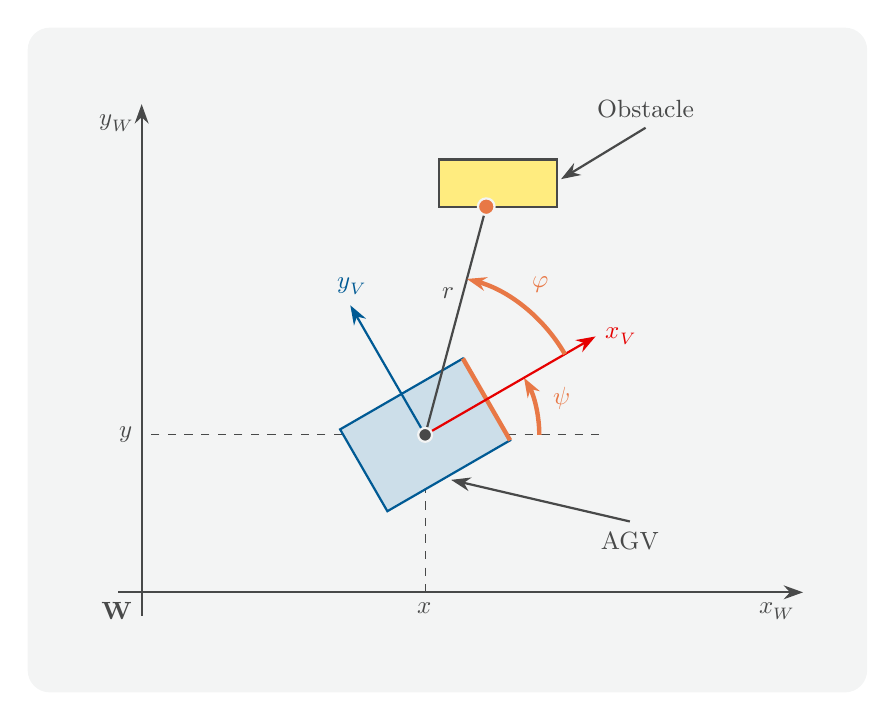
\begin{tikzpicture}[
    show background rectangle,
    background rectangle/.style={fill=my_lightgray, rounded corners=8pt},
    inner frame sep=0.8cm,
    annotation/.style={draw=my_darkgray, thick, -{Stealth[length=7pt, width=5pt]}},
    achse/.style={thick, -{Stealth[length=7pt, width=5pt]}}
]

    % Schematische Draufsicht, nicht maßstäblich.
    % Fahrzeugmitte C, Gierwinkel psi = 30 Grad, Messstrahl unter phi = 45 Grad
    % gegen die x_V-Achse, also unter 75 Grad gegen die x_W-Achse.
    \coordinate (O) at (0,0);
    \coordinate (C) at (3.6,2.0);
    \coordinate (P) at ($(C)+(75:3.0)$);

    % Weltkoordinatensystem W
    \draw[achse, draw=my_darkgray] (-0.3,0) -- (8.4,0)
        node[anchor=north east, font=\small, text=my_darkgray] {$x_W$};
    \draw[achse, draw=my_darkgray] (0,-0.3) -- (0,6.2)
        node[anchor=north east, font=\small, text=my_darkgray] {$y_W$};
    \node[font=\small\bfseries, text=my_darkgray, anchor=north east] at (O) {W};

    % Lage der Fahrzeugmitte in Weltkoordinaten
    \draw[draw=my_darkgray, thin, dashed] (C) -- (C |- O)
        node[anchor=north, font=\small, text=my_darkgray] {$x$};
    \draw[draw=my_darkgray, thin, dashed] (C) -- (C -| O)
        node[anchor=east, font=\small, text=my_darkgray] {$y$};

    % Hindernis mit getroffenem Punkt P auf seiner Unterkante
    \draw[fill=my_yellow, draw=my_darkgray, thick] ($(P)+(-0.6,0)$) rectangle ($(P)+(0.9,0.6)$);

    % Gierwinkel psi zwischen der Parallelen zur x_W-Achse und der x_V-Achse
    \draw[draw=my_darkgray, thin, dashed] (C) -- ($(C)+(2.3,0)$);
    \draw[draw=my_orange, ultra thick, -{Stealth[length=7pt, width=5pt]}]
        ($(C)+(1.45,0)$) arc[start angle=0, end angle=30, radius=1.45];
    \node[font=\small, text=my_orange] at ($(C)+(15:1.8)$) {$\psi$};

    % Fahrzeug, gedreht um psi: Umriss hellblau, Vorderkante orange
    \begin{scope}[shift={(C)}, rotate=30]
        \draw[fill=my_lightblue, draw=my_darkblue, thick] (-0.9,-0.6) rectangle (0.9,0.6);
        \draw[draw=my_orange, ultra thick] (0.9,-0.6) -- (0.9,0.6);
        % Fahrzeugkoordinatensystem F
        \draw[achse, draw=my_red] (0,0) -- (2.5,0)
            node[anchor=west, font=\small, text=my_red] {$x_V$};
        \draw[achse, draw=my_darkblue] (0,0) -- (0,1.9)
            node[anchor=south, font=\small, text=my_darkblue] {$y_V$};
    \end{scope}

    % Messstrahl des Laserscanners mit Entfernung r und Winkel phi
    \draw[draw=my_darkgray, thick] (C) -- (P);
    \node[font=\small, text=my_darkgray, anchor=east] at ($(C)!0.62!(P)$) {$r$};
    \draw[draw=my_orange, ultra thick, -{Stealth[length=7pt, width=5pt]}]
        ($(C)+(30:2.05)$) arc[start angle=30, end angle=75, radius=2.05];
    \node[font=\small, text=my_orange] at ($(C)+(52.5:2.4)$) {$\varphi$};
    \draw[fill=my_orange, draw=my_lightgray, thick] (P) circle (3pt);

    % Fahrzeugmitte
    \draw[fill=my_darkgray, draw=my_lightgray, thick] (C) circle (2.5pt);

    % Beschriftungen
    \draw[annotation] (6.4,5.9) -- ($(P)+(0.95,0.35)$);
    \node[font=\small, text=my_darkgray, anchor=south] at (6.4,5.9) {Obstacle};
    \draw[annotation] (6.2,0.9) -- ($(C)+(-60:0.66)$);
    \node[font=\small, text=my_darkgray, anchor=north] at (6.2,0.9) {AGV};

\end{tikzpicture}
\end{document}
